\chapter{Nuclear forces}\label{ch:nuclear_forces}

For low-energy nuclear physics,
the goal is to understand the structure and dynamics of systems
with nucleons as constituents.
Thus, a key input into any theoretical calculations of such systems
is the interactions between nucleons.
However, quantum chromodynamics (QCD),
the theory of the strong interaction,
is given in terms of quarks and gluons, not nucleons.
Moreover, at low energies the strong interaction coupling constant $\alpha_s(q^2)$ becomes large,
preventing a fundamental closed-form solution for the interactions between color-neutral hadrons.

As a result, various approaches to determining the interactions between nucleons
have been developed.
One such approach is the phenomenological expansion of the interaction between two nucleons
into terms with different spin, isospin, and angular-momentum dependences.
The (position- and momentum-dependent) strength of each of these terms is then fit to nucleon-nucleon scattering data,
giving rise to, for example, the AV18 potential~\cite{Wiri95AV18}.
This approach has several features that make it undesirable for \abinitio{} nuclear theory.
First, it does not connect to the underlying fundamental theory.
Second, this approach does not prescribe a way to arrive at consistent three-nucleon forces.
Additionally, the fitting procedure often includes scattering data at relatively high energies
when compared to the expected kinetic energy of nucleons in nuclei or nuclear matter,
making such phenomenological interactions highly non-perturbative.

In this chapter, we discuss chiral effective field theory
as an alternative to the phenomenological determination of nuclear forces
and the similarity renormalization group as a method to generally ``soften'' interactions
for many-body calculations.
Then we discuss some details regarding different bases
in which one can represent nuclear potentials.

\section{Nuclear forces from chiral effective field theory}

\begin{figure}[t!]
  \centering
  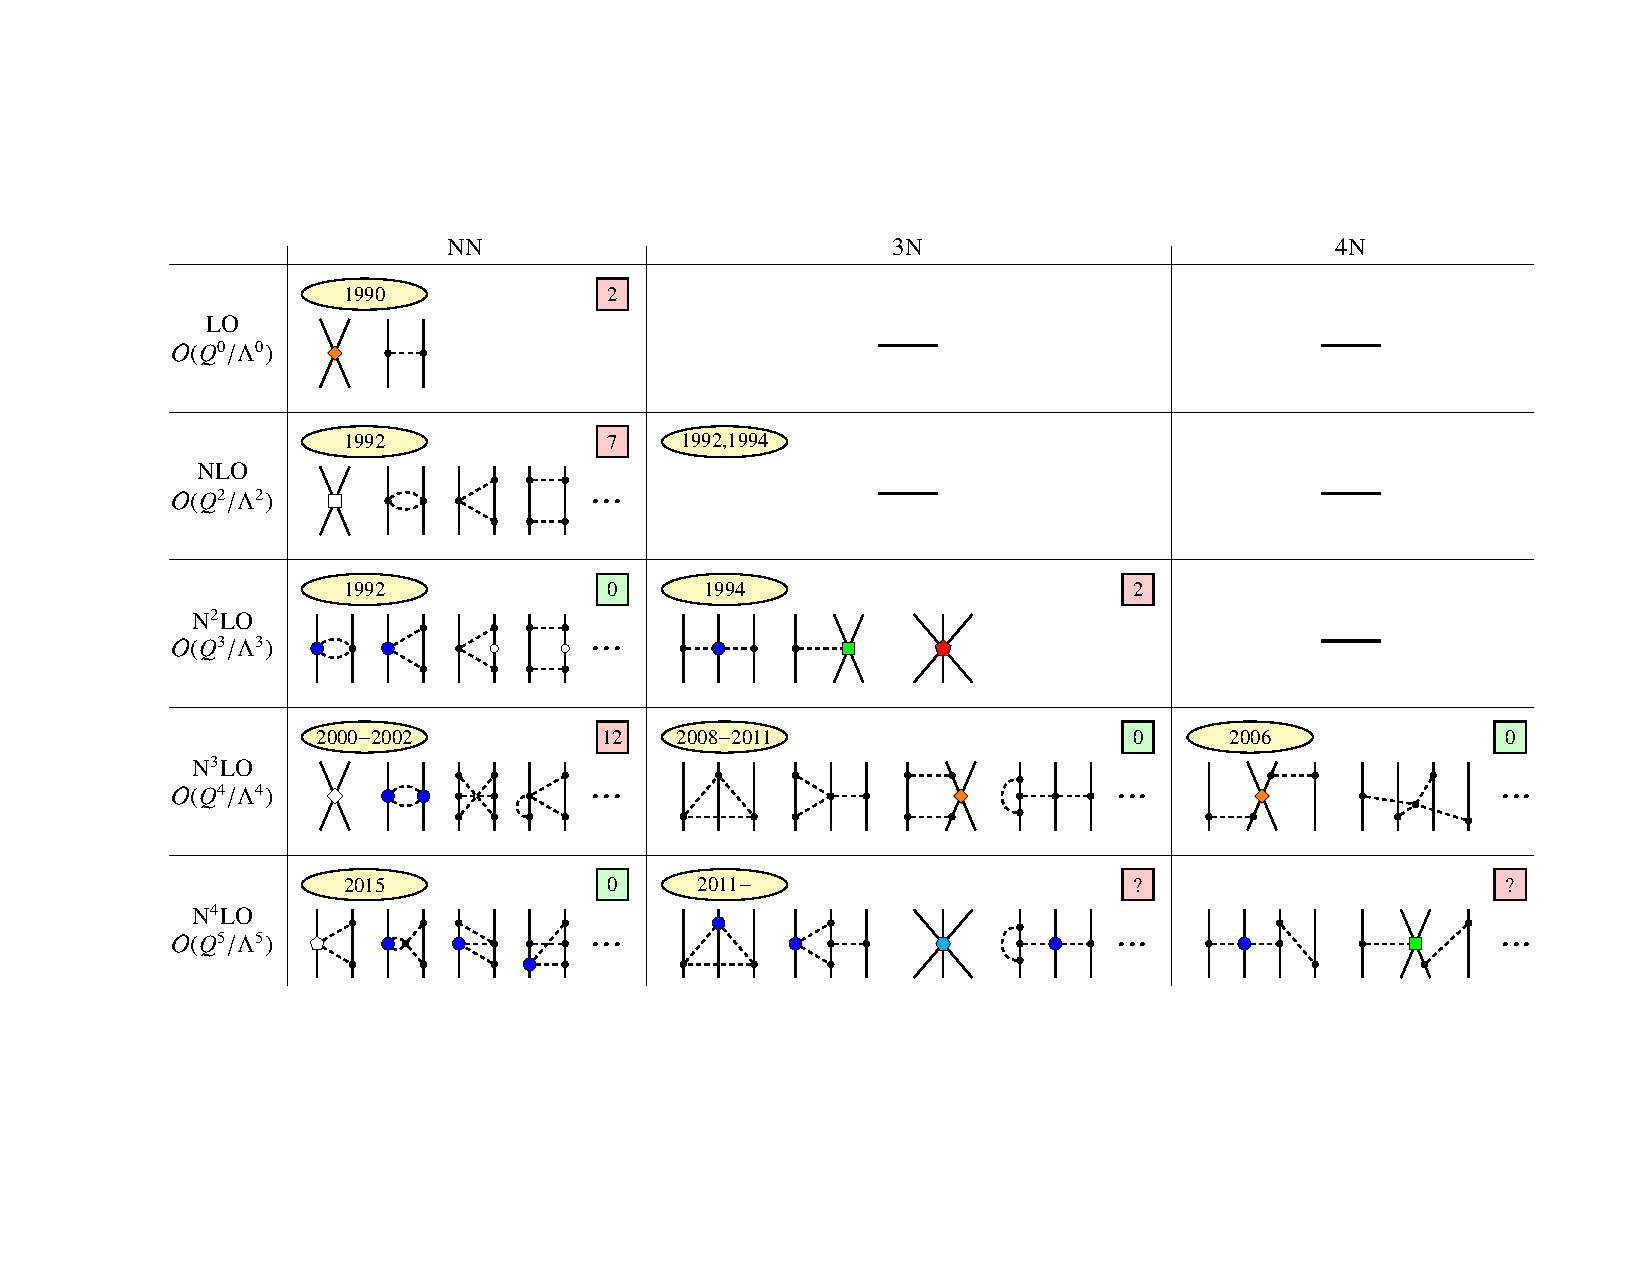
\includegraphics[width=1.0\textwidth]{thesis/doc/images/external/table_norefs.pdf}
  \caption[
    The contributions to NN, 3N, and 4N interactions in chiral EFT
    up to order \nfourlo{}.\@
    Solid lines indicate nucleon propagators.
    Dashed lines indicate pion propagators.
    The number of new LECs for the new interaction contributions at each new order
    is shown in the top right corner.
  ]{
    The contributions to NN, 3N, and 4N interactions in chiral EFT
    up to order \nfourlo{}.\@
    Solid lines indicate nucleon propagators.
    Dashed lines indicate pion propagators.
    The number of new LECs for the new interaction contributions at each new order
    is shown in the top right corner.
    Figure taken from Ref.~\cite{Hebe20habi}.
  }\label{fig:chiefttable}
\end{figure}

A modern approach to deriving nuclear potentials is chiral effective field theory.
The EFT approach allows one to systematically construct a field theory that approximates
a more fundamental theory in a low-energy domain~\cite{Epel08chiraleft,Mach11chiraleft,Hamm19nuceftreview}.
In this apppropriately chosen domain,
one can use the most efficient degrees of freedom to formulate the theory.
The construction of the theory relies on knowing the symmetries (exact and approximate) of the underlying theory.
Constructing the most general Lagrangian consistent with these underlying symmetries
yields the most general $S$-matrix~\cite{Wein78eft}.

To construct an effective field theory, one identifies the degrees of freedom one wants to work with
and identifies a high-momentum scale $\Lambda$ of the underlying theory that characterizes physics no longer resolved by the EFT~\cite{Hamm19nuceftreview}.
The EFT then should be an efficient, approximately complete description of the relevant physics
at momenta $Q$ small compared to $\Lambda$.
The chosen degrees of freedom are used to construct the most general Lagrangian consistent with the underlying symmetries,
which will have an infinite number of terms each with their own coefficients,
the so-called low-energy constants (LECs).
The EFT can then be used to calculate observables up to some precision in an expansion in $Q/\Lambda$,
made systematic by a power-counting approach.

For chiral EFT,
the underlying theory is QCD in the light-quark sector
(here this means only up and down quarks),
where the Lagrangian has an approximate chiral symmetry $\text{SU}{(2)}_L \times \text{SU}{(2)}_R$
in the limit of vanishing quark masses and no electroweak interactions~\cite{Hamm19nuceftreview}.
This symmetry is spontaneously broken,
giving rise to the pion as the Goldstone boson associated with the broken $\text{SU}{(2)}_A$ symmetry,
as well as explicitly broken by the non-zero quark masses~\cite{Page74chisymm}.
A logical choice of degrees of freedom is then nucleons and pions.
The high-momentum scale $\Lambda_b$ is set by the lightest meson not included in our degrees of freedom,
the $\rho$ meson with a mass of $m_{\rho}\approx 770 \mev$~\cite{Mach11chiraleft}.
The low-momentum scale is a collective scale given by $\text{max}(Q, m_{\pi})$.

The resulting potential contributions from chiral EFT have either explicit pion exchanges
or contact interactions with LECs describing short-range physics unresolved by the EFT,
as shown in Fig.~\ref{fig:chiefttable}.
The first consistent three-nucleon (3N) interactions appear at next-to-next-to-leading order (\ntwolo{}),
and the first four-nucleon (4N) interactions appear at next-to-next-to-next-to-leading order (\nthreelo{}).
Among the features that make EFTs so powerful is that they allow for clear error estimates~\cite{Furn15bayesuq,Epel14ekm1,Epel14ekm2},
given proper power counting,
by considering the order-by-order convergence of observables
and seeing that the orders left out due to a truncation at order $N$ should contribute something like
\begin{equation}
  \Delta O^{(N)} \sim O {\left(\frac{\text{max}(Q, m_{\pi})}{\Lambda_b} \right)}^{N+1}\,,
\end{equation}
where $O$ is the exact result for some observable of interest
(see Fig.~\ref{fig:chieft_uq}).

For potentials from chiral EFT,
at each order a finite number of undetermined LECs are introduced with the new contributions to the potential.
For nucleon-nucleon (NN) interactions, these can be determined by fitting to \textit{low-energy} scattering data.
For 3N interactions, the relevant LECs must be fit to three-body or four-body observables.
Typical choices for these observables at \ntwolo{}, where two three-body LECs, $c_D$ and $c_E$, need to be fit,
are the triton binding energy and either the triton half-life or the ${}^4\text{He}$ charge radius~\cite{Hebe20habi}.
Additionally, some contributions at later orders in the expansion only depend on LECs from previous orders.
For example, the 3N force contributions at \nthreelo{} require no new LECs to be fit.

\begin{figure}[t!]
  \centering
  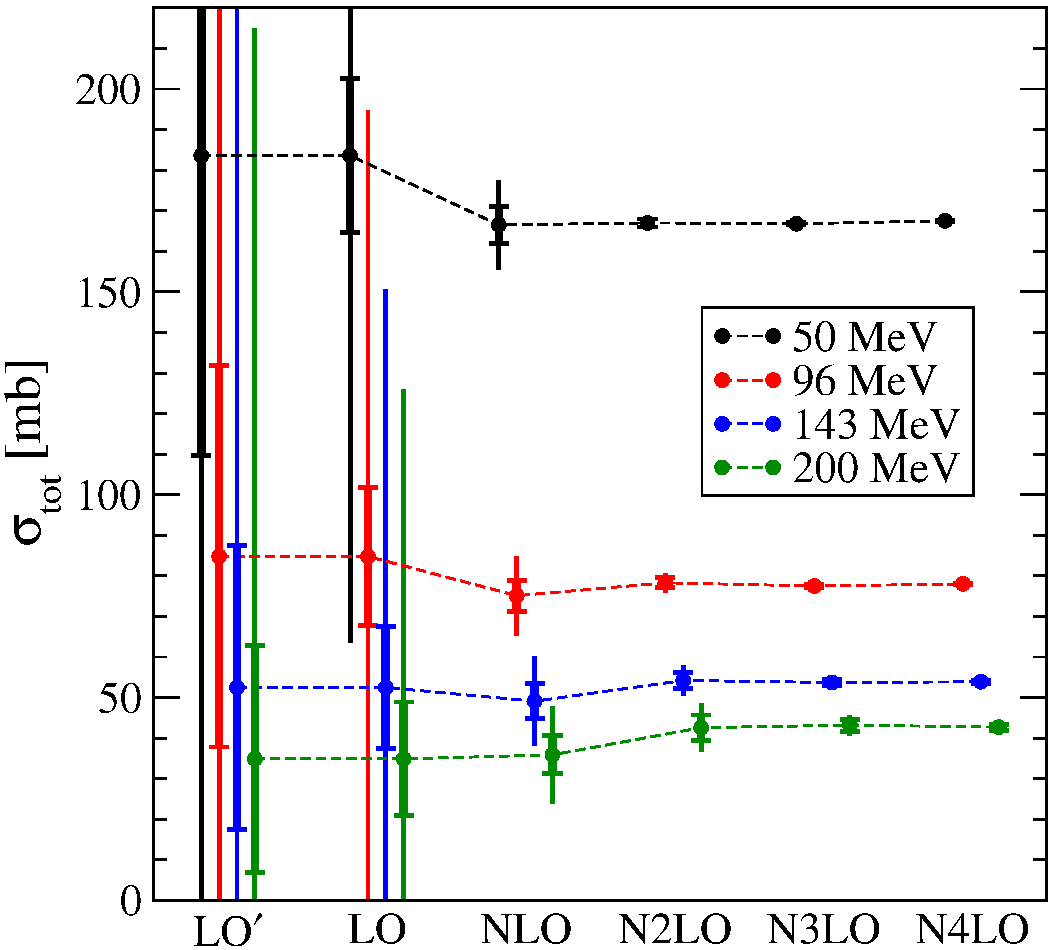
\includegraphics[width=0.5\textwidth]{thesis/doc/images/external/EKM_Tlab_together_setA_eps_approx0.pdf}
  \caption[
    The total proton-neutron scattering cross section
    calculated order by order at different energies
    using chiral potentials
    with 68\% and 95\% degree of belief intervals
    indicated by the thick and thin error bars
    obtained via Bayesian uncertainty quantification.
  ]{
    The total proton-neutron scattering cross section
    calculated order by order at different energies
    using potentials from Ref.~\cite{Epel14ekm2}
    with 68\% and 95\% degree of belief intervals
    indicated by the thick and thin error bars
    obtained via Bayesian uncertainty quantification~\cite{Furn15bayesuq}.
    Figure taken from Ref.~\cite{Furn15bayesuq}.
  }\label{fig:chieft_uq}
\end{figure}

Some comments are now in order regarding interactions as used in this thesis.
The derivation of potentials requires the explicit regularization of momenta
to make divergent integrals over intermediate momenta convergent.
This introduces a dependence on the regularization scheme and scale used,
which is an artifact of the finite order of our EFT.\@
Each additional order in the EFT cancels the scale dependence of the previous order,
and in the limit of infinite order all observables
should not depend on the cutoff scale and scheme used (within reason).
For every interaction used we state the order, the regularization scale,
and the family of interactions, which specifies the regularization scheme used.

We primarily use two families of interactions.
The first set is a family of interactions with NN interactions given up to \nthreelo{},
which was worked out by Entem and Machleidt in 2003~\cite{Ente03n3lonn}.
These interactions are denoted by EM when they are used.
The second set was worked out by Entem, Machleidt, and Nosyk in 2017
and provides NN interactions up to \nfourlo{}~\cite{Ente17n4lonn}.\@
These interactions are denoted by EMN.\@
From 2007 through 2011, the 3N interactions were worked out~\cite{Ishi07chi3n,Bern07chi3n1,Bern11chi3n2},
and the consistent
(in terms of power counting and regularization scheme)
3N potentials with these families up to \nthreelo{}
were presented in 2015 by Hebeler \textit{et al.}~\cite{Hebe15n3lo3n}.
At \nthreelo{}, the chiral power counting dictates the inclusion of 4N forces
(see Fig.~\ref{fig:chiefttable}).
However, this is generally \textit{not} done
because the inclusion of 4N forces in calculations is prohibitively expensive
and past results have shown that they contribute at the sub-1\%
level~\cite{Tews12neutronmatter4n,Schu18fourbody}.

Chiral EFT essentially resolves all of the shortcomings of phenomenological potentials mentioned previously.
There are still many open questions regarding the derivation of potentials via chiral EFT
and their consistent application in many-body calculations.
For example, there are multiple schools of thought regarding
what the correct power counting
for nuclear potentials is~\cite{Bean01pertchieft,Nogg05pertchieft,Epel18hownottorenormalize}.
Additionally, the uncertainties from the regularization scheme and scale for nuclear potentials
are still most likely dominant in many-body calculations.
However, the rapid expansion of the range of \abinitio{} calculations over the past two decades has been in no small part
due to the introduction of chiral potentials and the development of auxiliary tools to aid in their application
to many-body calculations.

\section{Similarity renormalization group evolution of nuclear forces}\label{sec:srg}

The similarity renormalization group (SRG) is a method that has been used to great success to ``soften'' nuclear interactions~\cite{Bogn06srg,Wegn94srg,Glaz93srg}.
The key idea of the SRG is the generation of a continuous unitary transformation of a given Hamiltonian $H$,
\begin{equation}
  H(s) = U(s) H U^{\dagger}(s)\,,
\end{equation}
where $s$ is the continuous flow parameter.
The resulting flow equation gives the evolution of the Hamiltonian
\begin{equation}\label{eq:srg_flow_eq}
  \frac{d H(s)}{ds} = [\eta(s), H(s)]\,,
\end{equation}
with $\eta(s) = U(s) d U^{\dagger}(s)/ ds$ and we choose $H(0) = H$.
An ``appropriate'' choice of the anti-Hermitian generator $\eta$
can generate a unitary transformation
such that $H(s)$ evolves, for example, towards a diagonal form.
This leads to a decoupling of low- and high-energy states in the Hamiltonian,
allowing for a truncation in momentum space or a discretized basis
without distorting low-energy observables.

The evaluation of the commutator in the SRG flow equation generates higher-body forces in the evolved Hamiltonian,
even if the initial Hamiltonian consists only of two- and three-body forces.
This means that the fully unitary SRG evolution of an $A$-body Hamiltonian
requires the evaluation of the flow equation in the $A$-body basis.
For all but the smallest systems, this is computationally infeasible.

A pragmatic approach uses the SRG restricted to the three-body space
to evolve two- and three-body nuclear forces to ``softer'' forms in momentum space~\cite{Hebe12srg3n},
reducing coupling between low- and high-energy states.
These evolved potentials are for few-body purposes equivalent to the un-evolved ones,
reproducing the few-body binding energies, radii, and NN phase shifts exactly.
After truncating the potentials, taking advantage of the decoupling,
the few-body observables remain essentially unchanged,
and the low-energy NN phase shifts are also preserved.

The typical choice for the generator in the so-called ``free-space'' SRG in nuclear applications is
\begin{equation}
  \eta(s) = [T_{\text{rel}}, H(s)]\,,
\end{equation}
where $T_{\text{rel}}$ is the relative kinetic energy of the two- and three-body systems.
In two-body Jacobi momentum coordinates, $T_{\text{rel}}$ is diagonal,
thus the right-hand side of the flow equation clearly has a fixed point if $H(s)$ is ever diagonal.
Evaluating the flow equation in momentum space in the two-body case for this choice for $\eta$ gives
\begin{equation}
  \frac{dV_2(s; p, p')}{ds} = - {(p^2 - {p'}^2)}^2 V_2(s; p, p') + \int dp'' (p^2 + {p'}^2 - 2 {p''}^2) V_2(s; p, p'') V_2(s; p'', p')\,,
\end{equation}
where $p$ and $p'$ are the incoming and outgoing Jacobi momenta of the two-body subsystem
(see Section~\ref{sec:jacobi_ms_rep}).
We also used the conventional choice of leaving the kinetic energy invariant under the SRG evolution.
Empirically, one can see that the first term dominates the evolution for far off-diagonal elements in nuclear applications,
and so
\begin{equation}
  V_2(s; p, p') \approx V_2(0; p, p') \exp(- s {(p^2 - {p'}^2)}^2)\,.
\end{equation}
Using a redefinition of the flow parameter
\begin{equation}
  \lambda = \frac{1}{s^{1/4}}\,,
\end{equation}
which has units of $\text{fm}^{-1}$ and evolves from $\lambda=\infty$ towards 0,
one can see that over the course of the evolution
off-diagonal parts of the potential outside a band of width $\lambda$ begin to be exponentially suppressed~\cite{Jurg07srgdec}.
Looking at Fig.~\ref{fig:srg_evolved_potential}, one can see that this is qualitatively true,
and the desired decoupling between low- and high-momentum states is achieved.

\begin{figure}[t]
  \centering
  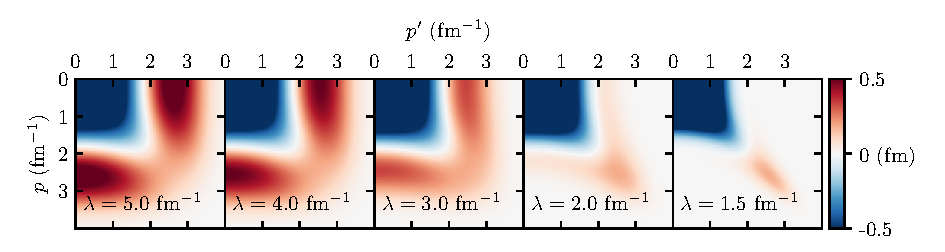
\includegraphics[width=\textwidth]{thesis/doc/images/vnn_srg_emn500_n3lo.pdf}
  \caption[
    An example of an SRG-evolved potential using the chiral EMN NN potential
    at \nfourlo{}
    in the ${}^3$S${}_1$ part of the ${}^3$S${}_1$-${}^3$D${}_1$ channel.
  ]{
    An example of an SRG-evolved potential using the chiral NN potential
    from Ref.~\cite{Ente17n4lonn} at \nfourlo{}
    in the ${}^3$S${}_1$ part of the ${}^3$S${}_1$-${}^3$D${}_1$ channel.
  }\label{fig:srg_evolved_potential}
\end{figure}

These softened interactions can then be fed into many-body frameworks,
which benefit strongly from the improved convergence with respect to model-space size.
However, the few-body evolution of potentials neglects induced $A$-body forces,
which do contribute in many-body calculations.
One way to probe the size of the missing many-body forces is to do calculations
with potentials evolved to different values of $s$ or $\lambda$
and see how much the calculated result depends on the renormalization scale.
A strong dependence would indicate significant missing contributions from many-body forces
while no dependence would indicate approximate renormalization group invariance,
which is ultimately the goal~\cite{Bogn09vlowk}.

\section{Representations of nuclear potentials}

The efficient representation of nuclear potentials exploits symmetries of the few-body system and the interactions.
In particular, for 3N forces,
where the potential can depend in principle on 18 parameters in momentum space
($\vec{k}_1$, $\vec{k}_2$, $\vec{k}_3$, $\vec{k}_{1}^{\prime}$, $\vec{k}_{2}^{\prime}$, $\vec{k}_{3}^{\prime}$),
simplifications afforded by these symmetries are essential
to being able to evaluate, store, and calculate with these potentials.

The essential symmetries of the free two- and three-nucleon systems
(from which the potentials are determined)
are~\cite{Hebe20habi}
\begin{itemize}
  \item conservation of the center-of-mass momentum of the system,
  \item independence on the center-of-mass momentum in the nonrelativistic regime,
  \item and rotational invariance.
\end{itemize}
Additionally, one can simplify things dramatically by making the assumption that the masses of all nucleons are the same,
a reasonable assumption given that the mass difference between the proton and neutron is less than a per mille~\cite{Hebe20habi}.
In this approximation in the absence of electroweak interactions,
the NN force would also be independent of isospin projection,
however the Coulomb interaction breaks this isospin charge symmetry.
Also, even without the Coulomb interaction,
the chiral EFT expansion explicitly breaks isospin charge symmetry at higher orders,
a result of it being constructed in a way
that systematically accounts for the breaking of approximate symmetries.

In the following, we discuss some possible representations of NN forces,
going from one of the representations most convenient for the evaluation of potentials
to the representation of choice for the many-body methods discussed in this thesis.
We mention along the way some of the analogous results for 3N forces.
A more thorough treatment of this topic can be found in Ref.~\cite{Hebe20habi}.

\subsection{Jacobi momentum space}\label{sec:jacobi_ms_rep}

Going from single-particle momenta to Jacobi and center-of-mass momenta,
like
\begin{align}
  \vec{k}_1, \vec{k}_2           & \rightarrow \vec{p}, \vec{P}_{2\text{N}}\,,           \\
  \vec{k}_1, \vec{k}_2,\vec{k}_3 & \rightarrow \vec{p}, \vec{q}, \vec{P}_{3\text{N}} \,,
\end{align}
allows one to factor out and ignore the center-of-mass degrees of freedom of the system.
The Jacobi and center-of-mass momenta are defined as
\begin{align}
  \vec{p}             & \equiv \frac{\vec{k}_1 - \vec{k}_2}{2}\,,            \\
  \vec{P}_{2\text{N}} & \equiv \vec{k}_1 + \vec{k}_2\,,                      \\
  \vec{q}             & \equiv \frac{2\vec{k}_3 - \vec{P}_{2\text{N}}}{3}\,, \\
  \vec{P}_{3\text{N}} & \equiv \vec{k}_1 + \vec{k}_2 + \vec{k}_3\,.
\end{align}
For NN forces, this gives us two-body states of the form
\begin{equation}
  \ket{\vec{p} s_1 m_{s_1} s_2 m_{s_2} t_1 m_{t_1} t_2 m_{t_2}}\,,
\end{equation}
where $s_i=1/2$, $m_{s_i}$, $t_i=1/2$, $m_{t_i}$ are the $i$-th particle's
spin, spin projection, isospin, and isospin projection, respectively.
In cases where explicit values of isospin projection are used,
we adopt the convention that for protons $m_t=1/2$ and for neutrons $m_t=-1/2$.

To take advantage of rotational invariance, one can decompose the potential into partial-wave channels,
with two-body states like
\begin{equation}
  \ket{p \left[l \left(s_1 s_2 \right) S \right] J m_{J} T m_{T}}\,,
\end{equation}
where $p$ is the magnitude of $\vec{p}$,
$l$ is the relative orbital angular momentum of the two-body system,
and $S$, $J$, $m_J$, $T$, $m_{T}$ are the
total spin, total angular momentum, total angular momentum projection, isospin, and isospin projection
of the two-body system.
The resulting potential
\begin{equation}
  \braket{p' \left[l' \left(s_{1}^{\prime} s_{2}^{\prime} \right) S' \right] J' m_{J}^{\prime} T' m_{T}^{\prime}
    | V_{2\text{N}} |
    p \left[l \left(s_{1} s_{2} \right) S \right] J m_{J} T m_{T}
  }\,
\end{equation}
is proportional to $\delta_{JJ'}\delta_{m_J m_{J'}}$ and independent of $m_J$ due to rotational invariance.
Additionally, antisymmetry under exchange of particle indices and parity conservation require
it to also be proportional to $\delta_{S S'} \delta_{T T'}$ with the additional constraints
\begin{align}
  {(-1)}^{l + S + T + 1} & = {(-1)}^{l' + S + T + 1} = 1\,, \\
  l - l'                 & = -2, 0, 2\,,
\end{align}
and charge conservation requires that it also is proportional to $\delta_{m_T m_{T'}}$.
For notational convenience, we sometimes collect the partial-wave quantum numbers of states
in a collective index $\alpha_2$,
giving the concise notation for 2N potentials
\begin{equation}
  \braket{p' \alpha_{2}^{\prime}|V_{2\text{N}}| p \alpha_2}\,.
\end{equation}

With this, the representation of NN forces has been reduced to two continuous variables, $p$ and $p'$,
and some strongly constrained partial-wave quantum numbers.
For 3N forces, there is similar simplification possible, yielding three-body states of the form
\begin{equation}
  \ket{p q \left[\left(l S\right) J \left(\ell s\right) j\right] \mathcal{J} \mathcal{M}_{\mathcal{J}} \left(T t\right) \mathcal{T} \mathcal{M}_{\mathcal{T}}}\,,
\end{equation}
where $p$, $l$, $S$, $J$, $T$ still refer to the two-particle subsystem as before,
$q$, $\ell$, $j$ are the Jacobi momentum, orbital angular momentum, and total angular momentum of the third nucleon
relative to the two-body subsystem center-of-mass,
and $s$ and $t$ are the spin and isospin of the third nucleon.
Here, the 3N potential is, among other things, independent of $\mathcal{M}_{\mathcal{T}}$.

\subsection{Jacobi harmonic-oscillator space}

The transformation to Jacobi harmonic-oscillator (HO) space follows quite simply.
Using the radial solutions to the isotropic three-dimensional harmonic oscillator with frequency $\hbar \Omega$,
one obtains
\begin{equation}\label{eq:jacobi_ho_twobody}
  \braket{n' \alpha_{2}^{\prime}|V_{2\text{N}}|n \alpha_2} = \int dp p^2 dp' {p'}^2 R_{n'l'}(p') R_{nl}(p)
  \braket{p' \alpha_{2}^{\prime}|V_{2\text{N}}|p \alpha_2}\,.
\end{equation}
The radial solutions are given by
\begin{equation}
  R_{n l}(p) = \sqrt{\frac{2(n!)}{{(m \hbar \Omega)}^{3/2} \Gamma(n + l + 3/2)}}
  {\left(\widetilde{p}\right)}^{l}
  \exp(- \widetilde{p}^2/2)
  L^{l + 1/2}_{n}\left(\widetilde{p}^2\right)\,,
\end{equation}
where $m$ is the nucleon mass, $\widetilde{p} \equiv p/\sqrt{m \hbar \Omega}$ is the dimensionless momentum,
and $L_{n}^{k}(x)$ are the generalized Laguerre polynomials.
For 3N forces, the Jacobi momenta $q$ and $q'$ must also be transformed, giving two more integrals.

In the infinite model-space limit, this transformation is exact,
and the dependence on the basis frequency $\hbar \Omega$ disappears.
However, for practical calculations a basis truncation $n_{\text{max}}$ must be introduced,
which implicitly introduces an ultraviolet (UV) cutoff and an infrared (IR) cutoff on the potential.
The UV cutoff is due to high frequencies requiring HO wave functions beyond the truncation to be resolved.
The IR cutoff is due to the basis frequency $\hbar \Omega$ setting the minimum frequency reproducable by wave functions in the basis.

For a given truncation,
the optimal $\hbar \Omega$ can be determined by making use of the variational principle,
which states that for the true ground state
the energy functional $E[\ket{\psi}]$ is stationary
under infinitesimal variations of $\ket{\psi}$.
In this case, one can look at the approximate ground state by solving
the two- or three-body system (for example, via exact diagonalization).
For the optimal $\hbar \Omega$, the ground-state energy will be minimal,
guaranteed by the variational principle to be no less than the true ground-state energy.
Many-body calculations are typically done with operators transformed
at several $\hbar \Omega$.
For energies the minimum result under this variation
is taken to be the result of the calculation,
but it is important to note that many many-body methods are \textit{not} variational.

\subsection{Single-particle harmonic-oscillator space}\label{sec:sp_ho}

Many many-body methods used in nuclear physics,
in particular also many-body expansion methods,
work with operators given in a single-particle basis as input.
This means we have a basis of single-particle states
\begin{equation}
  \left\{ \ket{a} \right\}
\end{equation}
spanning the one-body Hilbert space.
Then the set of product states
\begin{equation}
  \ket{a b} = \ket{a} \ket{b}
\end{equation}
spans the two-body Hilbert space.
At this point these states are not appropriately antisymmetrized.
At the end of this section,
we discuss how to recover the required antisymmetry under exchange of particle indices.

In our case, we work with the single-particle harmonic-oscillator basis with the same frequency $\hbar \Omega$
as used in the transformation above.
To be explicit, these states are of the form
\begin{equation}\label{eq:ho_sp_states}
  \ket{n_a \left(l_a s_a\right) j_a m_{j_{a}} t_a m_{t_a}}\,.
\end{equation}
The two-body single-particle states are then
\begin{equation}\label{eq:mscheme_twop_state}
  \ket{n_a \left(l_a s_a\right) j_a m_{j_{a}} t_a m_{t_a} n_b \left(l_b s_b\right) j_b m_{j_b} t_b m_{t_b}}\,,
\end{equation}
or, coupled to two-body total angular momentum $J$,
\begin{equation}\label{eq:jscheme_twop_state}
  \ket{n_a n_b \left[\left(l_a s_a\right) j_a \left(l_b s_b\right) j_b\right]J m_{J} t_a m_{t_a} t_b m_{t_b}}\,.
\end{equation}

To connect the states in Eq.~\eqref{eq:mscheme_twop_state} with those in Eq.~\eqref{eq:jacobi_ho_twobody},
one does a Talmi-Moshinsky transformation.
This connects the relative and center-of-mass excitation numbers, $n$ and $N$,
and orbital angular momentum numbers, $l$ and $L$,
with the single-particle excitation numbers, $n_a$ and $n_b$,
and orbital angular momentum numbers, $l_a$ and $l_b$.
The central object of this transformation is the harmonic-oscillator bracket
\begin{equation}
  \braket{n_a n_b (l_a l_b) \Lambda | n N (l L) \Lambda}\,,
\end{equation}
where both sets of orbital angular momenta have been coupled to total orbital angular momentum $\Lambda$.
The properties and evaluation of these brackets is discussed in detail in Refs.~\cite{Mosh59hobr,Buck96hobr}.
By appropriately decoupling and recoupling angular momenta
and applying the harmonic-oscillator brackets,
one arrives at NN potential matrix elements of the form
\begin{equation}\label{eq:unsymm_sp_me}
  \braket{ab | V_{2\text{N}} | cd}\,,
\end{equation}
where $a$, $b$, $c$, and $d$ are collective indices
that run over the single-particle states in Eq.~\eqref{eq:ho_sp_states}.

The matrix elements in Eq.~\eqref{eq:unsymm_sp_me}
do not obey the required antisymmetry of fermions under exchange of particle indices
since the product states $\ket{ab}$ are not antisymmetrized.
Restoring the required antisymmetry,
one obtains the antisymmetrized matrix elements
\begin{align}
  V_{2\text{N},abcd} & = \frac{1}{2}(1 - P_{ab})(1 - P_{cd})\braket{ab | V_{2\text{N}} | cd} \\
                     & = (1 - P_{cd}) \braket{ab | V_{2\text{N}} | cd}\,,
\end{align}
where $P_{ab}$ exchanges the indices $a$ and $b$ in the following expression.
The simplification above takes advantage of the symmetry
\begin{equation}
  \braket{ab | V_{2\text{N}} | cd} = \braket{ba | V_{2\text{N}} | dc}\,,
\end{equation}
arising due to the indistinguishability of the two particles.
In the next chapter, we develop the fundamentals of the formalisms
that use these matrix elements as input.
